\def\mytitle{MATRIX ANALYSIS USING PYTHON}
\def\myauthor{V.GOKULKUMAR}
\def\contact{velicharlagokulkumar@gmail.com}
\def\mymodule{Future Wireless Communication (FWC)}
\documentclass[10pt, a4paper]{article}
\usepackage[a4paper,outer=1.5cm,inner=1.5cm,top=1.75cm,bottom=1.5cm]{geometry}
\twocolumn
\usepackage{graphicx}
\graphicspath{{./images/}}
\usepackage[colorlinks,linkcolor={black},citecolor={blue!80!black},urlcolor={blue!80!black}]{hyperref}
\usepackage[parfill]{parskip}
\usepackage{lmodern}
\usepackage{tikz}
\usepackage{physics}
%\documentclass[tikz, border=2mm]{standalone}
%\usepackage{karnaugh-map}
%\documentclass{article}
\usepackage{tabularx}
%\usepackage{circuitikz}
\usepackage{enumitem}
\usetikzlibrary{calc}
\usepackage{amsmath}
\usepackage{amssymb}
\renewcommand*\familydefault{\sfdefault}
\usepackage{watermark}
\usepackage{lipsum}
\usepackage{xcolor}
\usepackage{listings}
\usepackage{float}
\usepackage{titlesec}
\providecommand{\mtx}[1]{\mathbf{#1}}
\titlespacing{\subsection}{1pt}{\parskip}{3pt}
\titlespacing{\subsubsection}{0pt}{\parskip}{-\parskip}
\titlespacing{\paragraph}{0pt}{\parskip}{\parskip}
\providecommand{\qfunc}[1]{\ensuremath{Q\left(#1\right)}}
\providecommand{\sbrak}[1]{\ensuremath{{}\left[#1\right]}}
\providecommand{\lsbrak}[1]{\ensuremath{{}\left[#1\right.}}
\providecommand{\rsbrak}[1]{\ensuremath{{}\left.#1\right]}}
\providecommand{\brak}[1]{\ensuremath{\left(#1\right)}}
\providecommand{\lbrak}[1]{\ensuremath{\left(#1\right.}}
\providecommand{\rbrak}[1]{\ensuremath{\left.#1\right)}}
\providecommand{\cbrak}[1]{\ensuremath{\left\{#1\right\}}}
\providecommand{\lcbrak}[1]{\ensuremath{\left\{#1\right.}}
\providecommand{\rcbrak}[1]{\ensuremath{\left.#1\right\}}}
\newcommand{\figuremacro}[5]{
    \begin{figure}[#1]
        \centering
        \includegraphics[width=#5\columnwidth]{#2}
        \caption[#3]{\textbf{#3}#4}
        \label{fig:#2}
    \end{figure}
}
\newcommand{\myvec}[1]{\ensuremath{\begin{pmatrix}#1\end{pmatrix}}}
\let\vec\mathbf
\lstset{
frame=single, 
breaklines=true,
columns=fullflexible
}
\thiswatermark{\centering \put(181,-119.0){
\includegraphics[scale=0.13]{iith_logo3}} }
\title{\mytitle}
\author{\myauthor\hspace{1em}\\\contact\\FWC22034\hspace{6.5em}IITH\hspace{0.5em}\mymodule\hspace{6em}Assignment}
\begin{document}
	\maketitle
	\tableofcontents
   \section{Problem}
 The area of the quadrilateral formed by the tangents at the end points of latus rectum to the ellipse \begin{align}
\frac{x^2}{9}+\frac{y^2}{5}=1
  \end{align}
\section{Construction}
  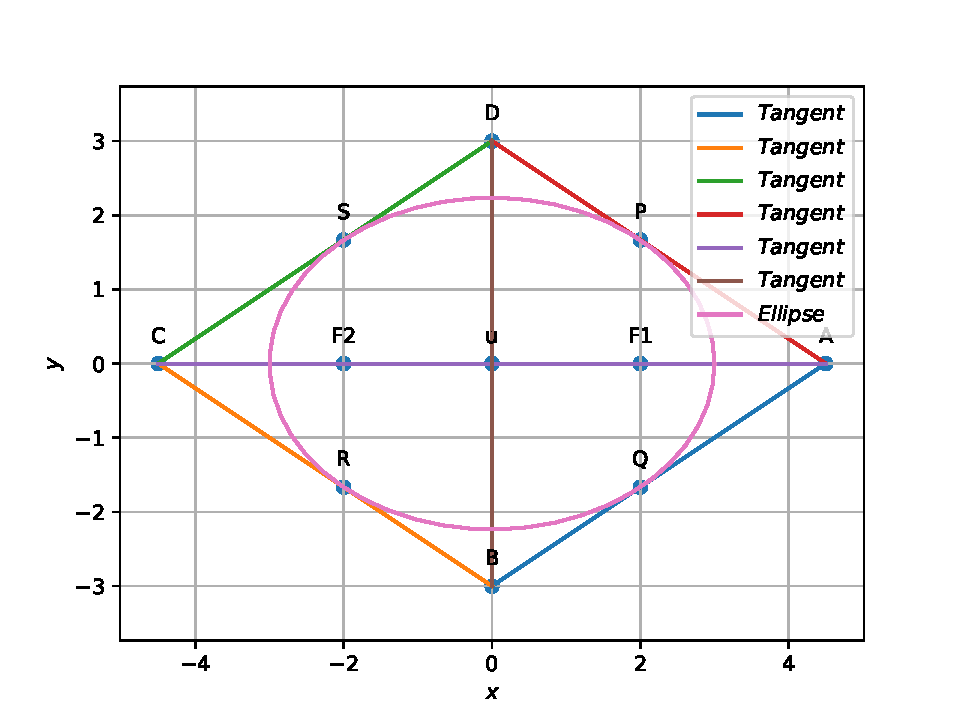
\includegraphics[scale=0.47]{matrix.pdf}
  	\begin{center}
  Figure of construction
  	\end{center}
  \section{Solution}

Ellipse equation : \begin{align}
\frac{x^2}{9}+\frac{y^2}{5}=1
  \end{align}
The standard equation of the conics is given as :
\begin{align}
\vec{x}^{\top}\vec{V}\vec{x}+2\vec{u}^{\top}\vec{x}+f=0
\end{align}
\begin{center}
Below python code realizes the above construction :
\fbox{\parbox{8.5cm}{\url{https://github.com/velicharlagokulkumar/FWC_module1/blob/main/matrices/conics/codes/matrix.py}}}
\end{center}
 The steps for constructing above figure are :
\begin{enumerate}
 \item Generate a Ellipse with vertex $\vec{u}$
 \item Find the ends of latus rectum  
 \item Find the equations of the tangent at one end of latus rectum and use that to find the X-intercept and Y-intercept
  \item Find the Area of the quadrilateral formed by all the tangents
\end{enumerate}
The given ellipse can be expressed as conics with \\parameters
\begin{align}
	\lambda_1&=5,\lambda_2=9 \\ \vec{V} &= \myvec{	\lambda_1& 0 \\
			          0 & \lambda_2}  
		    , \vec{u} = \myvec{0 \\0}, f = -45
	\end{align}
	Eccentricity:
	\begin{align}
	 e&=\sqrt{1-\frac{\lambda_1}{\lambda_2}}\\
	 \implies e&=2/3
	 \end{align}
	 Focus:
	 \begin{align}
	 f0&=-f,\vec{e1} = \myvec{1 \\0}\\
	 \vec{F}&= \pm e\sqrt{\frac{\abs{f_0}}{\lambda_2\brak{1-e^2}}}\\
	 	 \vec{F1}&=  e\sqrt{\frac{\abs{f_0}}{\lambda_2\brak{1-e^2}}}\vec{e}_1\\
	 	 \vec{F2}&= - e\sqrt{\frac{\abs{f_0}}{\lambda_2\brak{1-e^2}}}\vec{e}_1\\
	 \implies \vec{F1}&=\myvec{2\\0},\vec{F2}=\myvec{-2\\0}
	 \end{align}
	 Length of latus rectum:
	 \begin{align}
	 l&=2\frac{\sqrt{\abs{f_0\lambda_1}}}{\lambda_2}\\
	  l/2&=\frac{\sqrt{\abs{f_0\lambda_1}}}{\lambda_2}\implies 5/3
	  \end{align} 
End points of latus rectum:
\begin{align}
\vec{P}&=\myvec{F\\l/2},\vec{Q}=\myvec{F\\-l/2}\\\vec{R}&=\myvec{-F\\l/2},\vec{S}=\myvec{-F\\-l/2}
\end{align}
\begin{align}
\vec{P}&=\myvec{2\\5/3},\vec{Q}=\myvec{2\\-5/3}\\\vec{R}&=\myvec{-2\\5/3},\vec{S}=\myvec{-2\\-5/3}
\end{align}
  %  The input parameters for this construction are
%\begin{center}
%\begin{tabular}{|c|c|c|}
%	\hline
%	\textbf{Symbol}&\textbf{Value}&\textbf{Descriptio%n}\\
%	\hline
%	$\vec{F1}$ &\myvec{2\\0}& Focus\\
%	\hline
%   $\vec{F2}$ &\myvec{-2\\0}& Focus\\
%	\hline
% $\vec{P}$&\myvec{2\\5/3}& End of latus rectum\\
%	\hline
%	 $\vec{Q}$&\myvec{2\\-5/3}& End of latus rectum\\
%
%\hline
%	 $\vec{R}$&\myvec{-2\\-5/3}& End of latus %rectum\\
%	\hline
%	 $\vec{S}$&\myvec{-2\\5/3}& End of latus rectum\\
%	\hline
%\end{tabular}
%\end{center}
Equation of tangent to (3) at the point of contact $\vec{p}$, is 
\begin{align}
  \brak{\vec{V}\vec{p}+\vec{u}}^{\top}\vec{x}+\vec{u}^{\top}\vec{p}+f = 0 \\
 \brak{\myvec{5 & 0 \\
		 0 & 9}\myvec{2 \\
		              \frac{5}{3}}+\myvec{0\\0}}^{\top}
		               \myvec{x \\
		                      y}+\myvec{0 \ 0}\myvec{2 \\
		                             \frac{5}{3}}-45=0\\
\myvec{10\\15}^{\top}\myvec{x \\
		                    y}-45=0
\end{align}
let
		\begin{align}
	    \vec{n}^{\top} = \myvec{10 \\ 15},c=45
	    	\end{align}
	    X-intercept :
	    \begin{align}
	    \frac{c}{n^{\top}e1}
	    \end{align}
	    Y-intercept : 
	    \begin{align}
	    \frac{c}{n^{\top}e2}
	    \end{align}
	    \begin{align}
	    \vec{A} = \myvec{9/2 \\ 0},  
	    \vec{B} = \myvec{ 0 \\ -3}\\
	    \vec{C} = \myvec{-9/2 \\ 0},    
	    \vec{D} = \myvec{ 0 \\ 3}\\
		\end{align}
Letting,
\begin{align}
\vec{v1}=\vec{u}-\vec{D}\\
\vec{v2}=\vec{u}-\vec{A}
\end{align}		
	Area of the $\Delta$DuA is given by 
	\begin{align}
&=\frac{1}{2}\norm{\vec{v1}\times\vec{v2}}
\end{align}
	Area of the of quadrilateral ABCD is given by 
	\begin{align}
&=4\times\frac{1}{2}\norm{\vec{v1}\times\vec{v2}}
\end{align}
\begin{center}
    $\therefore$The area of quadrilateral ABCD=27 sq.units\\
\end{center}
\textbf{termux commands :}
\begin{lstlisting}
bash sh3.sh............using shell command
\end{lstlisting}

\end{document}
ent}
